%----------------------------------------------------------------------------------------
%	FORTHCOMING RESEARCH
%----------------------------------------------------------------------------------------

\section*{Strength, Weakness and Forthcoming Research}

\subsection*{Strengths}
The penalized-likelihood approaches brought up by this paper have two advantages over standard approach who use greedy stepwise regression for model selection and do parameter estimation based on the selected model.  First, greedy stepwise regression is computationally more challenging than penalized-likelihood methods.  Second, instead of determining neighborhood set for each $X_j$ locally through hypothesis testing at some level $\alpha$, which has long been recognized that this procedure does not correctly take account of the multiple comparisons involved, penalized-likelihood methods can globally determine graph structure avoid involving multiple dependent hypothesis tests.  Many other methods like the greedy stepwise regression approach, model selection and parameter estimation are done seperately.  However, penalized-likelihood estimators have precluded the discrete nature of such procedures which often leads to instability of the estimator.  In most cases, since the estimators are based on maximum likelihood estimator the solutions of the penalized-likelihood estimators are continuous.  Such continuity can ensure the stability of estimators.  

Compared with the method proposed by Meinshausen \& Bühlmann (2006), the paper's penalized-likelihood methods natrually incorporate the symmetry and positive-definiteness constraints in the estimation of the concentration matrix.  In addition, since the loss function used by Meinshausen \& Bühlmann (2006) is different from the quadratic approximation to the loglikelihood, the likelihood based approaches proposed by the paper are expected to be more efficient.
  

%\begin{figure}
%\centering
%\includegraphics[width=1\textwidth]{compare.png}
%\caption{\label{fig:compare}(a) Lasso-type estimator (b) garrote type estimator for the case of p = 2.}
%\end{figure}


The paper proposed two type of penalized likelihood methods.  One is LASSO-type method and the other is `nonnegative garrote' type method.  From the example provided in the second section of the paper, it seems garrote-type method has more advantages over LASSO-type method.  As the MLE estimator's absolute value become larger and larger, approaching to 1, the garrote-type estimator tends to have relatively smaller penalty over the MLE estimator than LASSO estimator if both tuning parameter are well choosed.  For those entries that MLE estimators are close to 0, the LASSO-type method tends to have smaller penalty than garrote-type estimator.  Since the goal we have here is to achieve sparse structure and in the mean time provide more precise estimates as possible, if a good initial estimator is available, garrote-type estimator is more ideal than LASSO-type estimator.  Also, the asymptotic properties for garrote-type estimator are better than those for LASSO-type estimator.  The garrote-type estimator enjoys the so-called oracle property: it selects the right graph with probability tending to one and at the same time gives a root-n consistent estimator of the concetration matrix.  From the simulation result provided in the six section of the paper, for garrote-type estimator, using MLE estimator as an initial estimator seems already good enough to compete with LASSO-type estimator.


\subsection*{Weaknesses}

An obvious weakness of the penalized-likelihood approaches in the paper is that they achieve sparsity by adding penalty term to the loglikelihood to get a shrinkage estimator for the concentration matrix globally.  To achieve sparsity, we may want to add penalty to make those entries who close to 0 to be shrinked to 0.  But for those entries who significantlly non-zero, we may want more accurate estimation of their true values.  The shrinkage estimator simultaneously penalize all entries in the matrix at an almost same level, so for those entries who significantlly non-zero, penalized-likelihood estimator may lose much more accuracy than the MLE estimator.

Another weakness is that for garrote-type estimator, we need a good initial estimator.  As shown in Figure 1, although garrote-type estimator penalize less when r far from 0, the distance between garrote-type estimator and MLE estimator is, in genral, larger than we expected.

\subsection*{Possible future directions}

\begin{center}
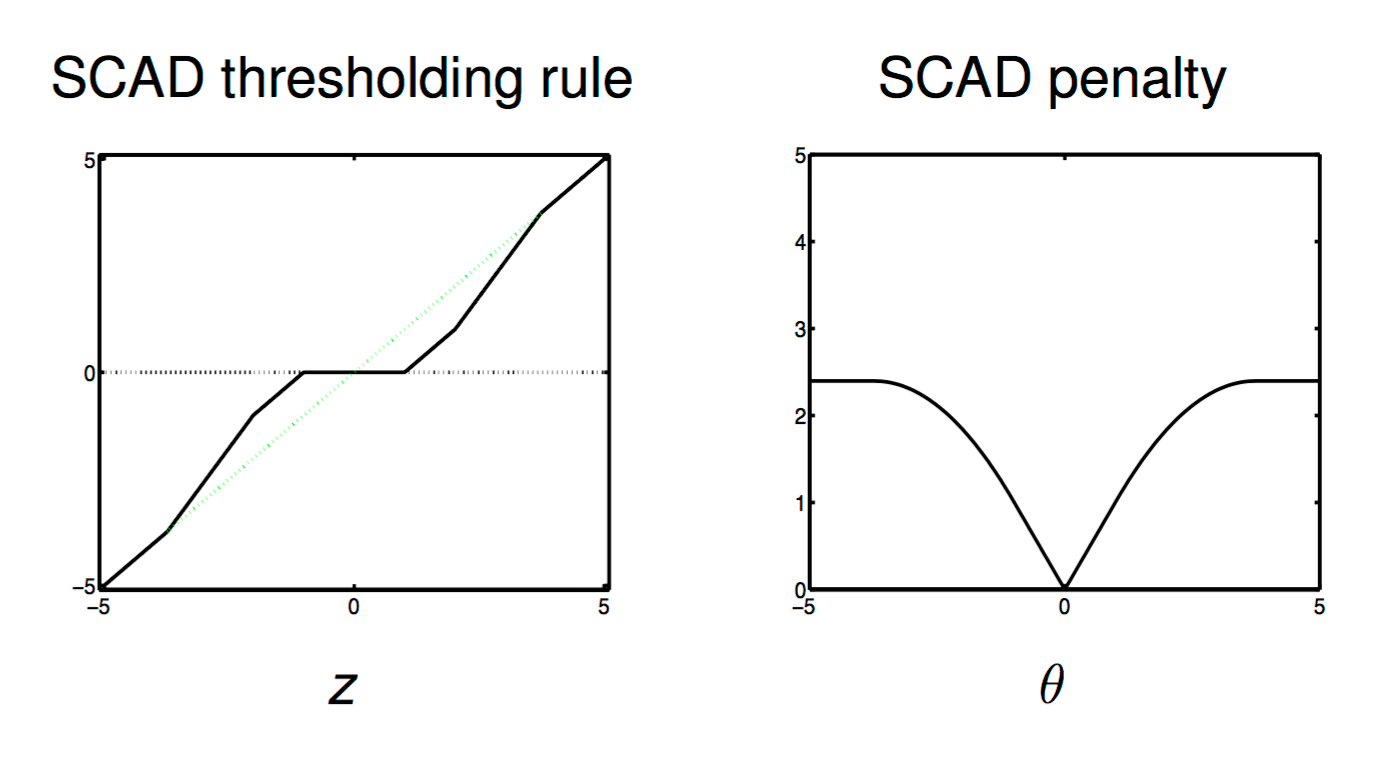
\includegraphics[width=0.75\linewidth]{scad}
\captionof{figure}{\color{Green} (a) Lasso-type estimator, (b) garrote-type estimator}
\end{center}

As mentioned above, we do not want a shrinkage estimator simultaneously penalize all entries in the matrix at a same level.  An ideal estimator we want could be that penalizes entries that are more close to 0 more severely than penalizing entries that are significantly non-zero.  One straightforward idea would be that we use penalized-likelihood methods to find those 0 entries in the estimator and for other entries we use the MLE estimated values as our estimator.  This idea is reasonable, but if we do this, our estimator would have a `jump' respect to estimated values.  For example, if we do this, it is very likely our estimated concentration matrix do not have entry value that falls between $(0, \alpha]$ ($\alpha$ is a value that close to 0) since all values smaller than $\alpha$ will be penalized to 0.  Also, we have to find a reasonable thresholding for doing this.  To avoid this situation, the idea of modifying LASSO penalty by SCAD penalty proposed by Jianqing Fan (1997) can be applied here.

$$P_{\tilde{\lambda}}^{scad} (\boldsymbol{\beta}) = ∑_{j=1}^p p_{\tilde{\lambda},j}^{scad} (|\beta_j|), \quad \tilde{\lambda} = (\lambda, s),$$

A SCAD penalty in regression has properties similar to what we want here.  From the Figure 2 we can find that SCAD penalty gives more sever penalty to larger coefficients than smaller coefficients in regression.  We can actually borrow the idea from the SCAD penalty to define a SCAD-type penalty to relpace the LASSO-type penalty term used in the paper which penalize more on entries whose MLE estimator close to 0 and penalize little on significantlly non-zero entries.